\documentclass[12pt,a4paper]{article}
\usepackage{rmpackages}																% usual packages
\usepackage{rmtemplate}																% graphic charter
\usepackage{rmexocptce}																% for DS with cptce eval

%\cfoot{} 													% if no page number is needed
%\renewcommand\arraystretch{1.5}		% stretch table line height

\begin{document}

\begin{header}
Les défis confinés -- Épisode 7
\end{header}

\section*{De quelle couleur sont les étoiles les plus chaudes}

\begin{multicols}{2}
\begin{center}
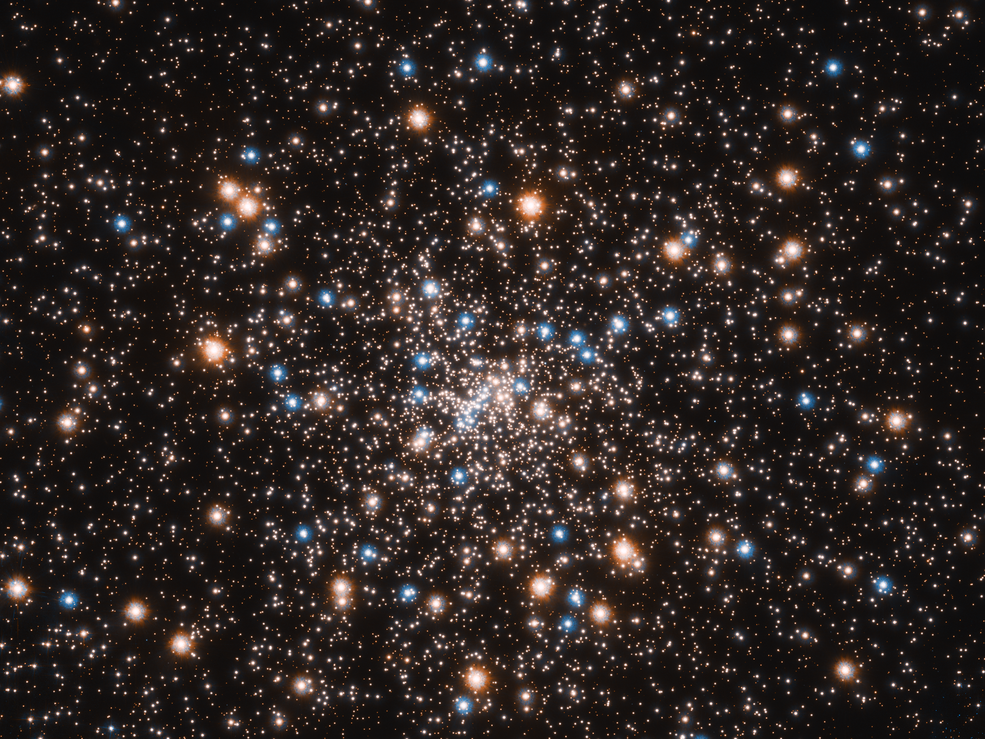
\includegraphics[trim=0 130 0 130, clip, width=\linewidth]{images/hubble_globular_cluster.png}
\end{center}

Comme le filament d'une ampoule ou une barre de métal chauffée à blanc, les étoiles sont des corps chauds (très chauds) qui émettent de la lumière.

On veut établir le lien entre la température d'une étoile et sa couleur, ce qui permet par exemple d'étudier précisément des étoiles pourtant situées très loin de nous.
\end{multicols}

\begin{enumerate}
\item \anarai{}
\label{quest:hyp}

La photo ci-dessus a été prise par le télescope spatial Hubble.
On peut l'observer en détail en cliquant \href{https://www.nasa.gov/feature/goddard/2021/hubble-uncovers-concentration-of-small-black-holes}{ici}.
On y voit d'innombrables étoiles.

À votre avis, lesquelles sont les plus chaudes : les bleues, les rouges ou plutôt les blanches ?
Justifier.

\item \app{} \anarai{}

La simulation interactive ci-dessous permet d'obtenir le spectre d'un corps chaud (comme une étoile) en fonction de sa température :

\href{https://phet.colorado.edu/sims/html/blackbody-spectrum/latest/blackbody-spectrum\_fr.html}{https://phet.colorado.edu/sims/html/blackbody-spectrum/latest/blackbody-spectrum\_fr.html}

On peut changer la température du corps avec le thermomètre situé à droite. 
La température est ici indiquée en kelvin (K) mais avec les valeurs utilisées ici, cette unité est presque équivalente aux degrés Celsius (\degree C).

Le graphe représente l'intensité lumineuse émise par le corps en fonction de la longueur d'onde donnée en micromètres.
On peut modifier les échelles des axes avec les loupes 
\includegraphics[height=0.75\baselineskip]{images/zoom_out.png} et 
\includegraphics[height=0.75\baselineskip]{images/zoom_in.png}.

\begin{enumerate}
\item Pour une température de \unit{3\,000}{K}, entre le rouge et le bleu, quelle couleur est émise avec le plus d'intensité ?

\item Et pour une température de \unit{10\,000}{K} ?

\item Comment évolue la composition du spectre en fonction de la température ?
\end{enumerate}
\end{enumerate}


\begin{enumerate}[resume]
\item \anarai{}

Les images ci-dessous montrent la couleur et les spectres de quelques étoiles \og proches \fg{}.

Classer ces étoiles de la plus froide à la plus chaude.

\textit{On peut vérifier la réponse à l'aide de l'étoile située en haut de la simulation.} \thumbsup

\item \val{}

Ces observations confirment-elles votre hypothèse de la question~\ref{quest:hyp} ?
\end{enumerate}

\newpage
\begin{center}
\newcommand{\localheight}{75 pt}
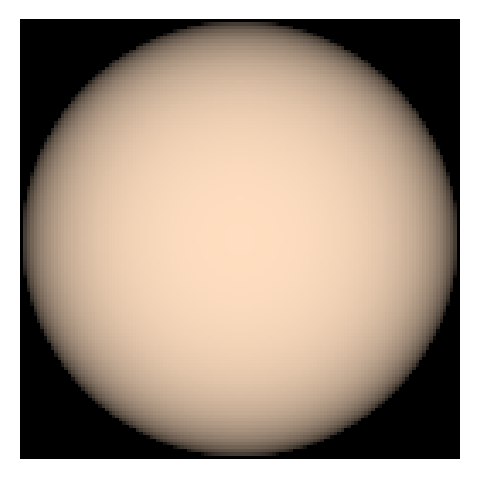
\includegraphics[height=\localheight]{images/star_tau_ceti.png}

\includegraphics[height=\localheight]{images/spectrum_star_tau_ceti.png}

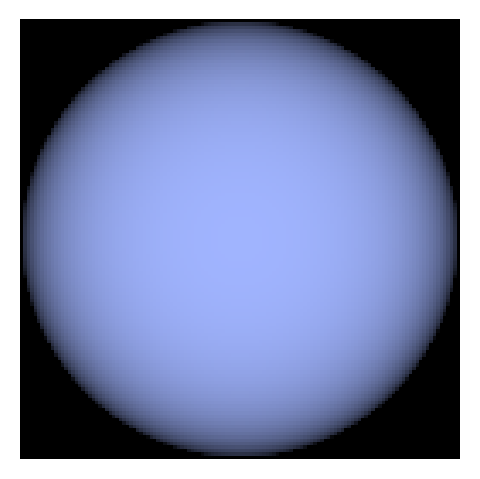
\includegraphics[height=\localheight]{images/star_rigel.png}

\includegraphics[height=\localheight]{images/spectrum_star_rigel.png}

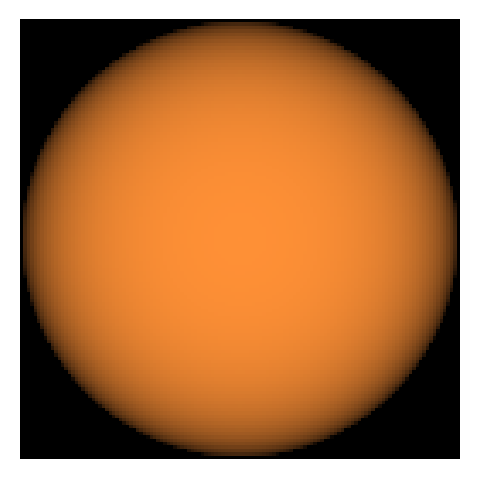
\includegraphics[height=\localheight]{images/star_proxima_centauri.png}

\includegraphics[height=\localheight]{images/spectrum_star_proxima_centauri.png}
\end{center}

\section*{Vitesse de la lumière}

\begin{enumerate}
\item \rea{}

Le Soleil se situe à une distance $d = \unit{1\dcoma50 \times 10^{11}}{m}$ de la Terre.
Sa lumière met un temps $\Delta t$ égal à 8 minutes et 20 secondes à nous parvenir.
Calculer la vitesse de la lumière notée $c$ avec ces valeurs.

\item \val{}

Votre valeur est-elle en accord avec la valeur de référence : $c=\unit{299\,792\,458}{m/s}$.

\end{enumerate}

\end{document}

\section*{Un spectroscope maison}

Pour obtenir le spectre d'une source de lumière, il faut un élément dispersif : un \textbf{prisme} ou un \textbf{réseau}.
Un réseau est une plaque transparente sur laquelle sont gravées de très fines lignes.
Certains DVD peuvent servir de réseau de fortune : c'est le cas des DVD-R.
Il est alors possible de réaliser un spectroscope maison.

Si le cœur vous en dit, vous pouvez réaliser le votre en suivant ce tutoriel :

\noindent
\href{http://toysfab.com/2018/03/fabriquer-un-spectrometre-avec-votre-smartphone/}{http://toysfab.com/2018/03/fabriquer-un-spectrometre-avec-votre-smartphone/}